%%%%%%
%$Autor: Shamsa Hasan$
%$Dateiname: RTC.tex$
%$Beschreibung: Beschreibung einer Echtzeituhr$
%%%%%%



%
%\chapter{\ac{rtc}}\label{RTC}
%
%\section{Einleitung}
% 
% Eine \ac{rtc} ist eine elektronische Komponente zur präzisen Zeitmessung, 
% die in zahlreichen Anwendungen eingesetzt wird. 
% Sie stellt sicher, dass elektronische Systeme auch nach einem Neustart oder Spannungsverlust 
% die korrekte Uhrzeit beibehalten. 
% Dies wird durch eine kontinuierliche Stromversorgung, 
% typischerweise über eine Knopfzellenbatterie, gewährleistet 
% (vgl. Abbildung~\ref{fig:rtc}). 
% 
% Im Gegensatz zur systeminternen Zeitmessung arbeitet die \ac{rtc} 
% unabhängig von der Hauptstromversorgung und zeichnet sich durch einen sehr geringen Energieverbrauch aus. 
% Neben der Uhrzeit kann sie auch das Datum und den Wochentag erfassen. 
% Dadurch wird ihr Einsatz insbesondere in Embedded-Systemen, 
% Computern und IoT-Anwendungen unverzichtbar. 
% 
% Die \ac{rtc} bildet somit eine wesentliche Grundlage für Systeme, 
% in denen zeitabhängige Prozesse, Protokollierungen oder Ereignissteuerungen erforderlich sind. 
% \cite{white2011}
% 
%\begin{center}
%	
\includegraphics[width=0.7\linewidth]{RTC/RTC}
%	\captionof{figure}{\ac{rtc} \cite{seeedstudio:2020}}
%	\label{fig:rtc}
%\end{center}
% 
%
%
%\section{Technische Spezifikationen}
%
%Die folgende Tabelle \ref{tab:rtc} zeigt die wichtigsten Spezifikationen der RTC auf einen Blick. Besonders hervorzuheben ist die geringe Stromaufnahme, die ihren Einsatz in batteriebetriebenen Geräten begünstigt. Die Größe des Moduls beträgt~$140 mm\times$85~mm $~\times10mm$.
%
%\begin{center}
%	\captionof{table}{Technische Daten des  RTC-Moduls DS1307 \cite{analog2008}}
%	\label{tab:rtc}
%	\begin{tabular}{|l|p{8cm}|}
%		\hline
%		IC Chip & DS1307 \\
%		\hline
%		Operating Voltage & 3.3 - 5 V \\
%		\hline
%		Max Stromaufnahme (aktiv) & 200 µA \\
%		\hline
%		Max Stromaufnahme (standby) & 2 µA \\
%		\hline
%		Zeitgenauigkeit & ±2 ppm \\
%		\hline
%		Betriebstemperatur & -40 bis 85°C \\
%		\hline
%		Batteriebackup & CR2032 \\ 
%		\hline
%		Abmaße & $140 mm \times 40 mm$ $\times 10 mm$ 
%	\end{tabular}
%\end{center}
%
%
%
%
%\begin{center}
%	\begin{tikzpicture}
%		% RTC Modul
%		\draw[fill=blue!50!black] (0,0) rectangle (5,3);
%		\draw[fill=white] (0.5,0.5) rectangle (1.25,2.5);
%		
%		\draw[fill=white!70!black](0.85,2.25) circle (0.1);
%		\draw[fill=white!70!black] (0.85,1.75)  circle (0.1);
%		\draw[fill=white!70!black](0.85,1.25) circle (0.1);				\draw[fill=white!70!black] (0.85,0.75) circle (0.1);
%		
%		
%		\node[anchor=east] at (0,2.25) {\tiny SDA};
%		\node[anchor=east] at (0,1.75) {\tiny SCL};
%		\node[anchor=east] at (0,1.25) {\tiny GND};
%		\node[anchor=east] at (0,0.75) {\tiny VCC};
%		
%		% Batteriehalter (runde Darstellung, auf dem Modul)
%		\draw[fill=gray!50!black] (3.5,1.5) circle (1);
%		\node[white] at (3.5,1.5) { CR2032};
%		
%
%		
%	\end{tikzpicture}
%	\captionof{figure}{RTC-Modul DS1307 nach \cite{seeedstudio:2025} }
%		\label{rtctixz}
%\end{center}
%
%\section{Anwendungen der RTC in verschiedenen Bereichen}
%
%\ac{rtc}s werden in einer Vielzahl von Anwendungen eingesetzt, darunter:
%
%- \textbf{Computer}: Für die Erhaltung der Uhrzeit und des Datums.\\
%- \textbf{Embedded Systems}: Als Zeitbasis für zeitabhängige Prozesse.	\\
%- \textbf{IoT-Geräte}: Zur Zeitstempelung von Ereignissen für Synchronisationszwecke. \\
%- \textbf{Akkubetriebene Geräte}: Minimierung des Stromverbrauchs während Standby-Phasen. \\
%- \textbf{Messgeräte}: Präzise Zeitmessungen ohne ständige Verbindung zu externen Stromquellen. \\
%
%Durch ihre vielseitige Anwendbarkeit und die Fähigkeit, kontinuierlich Zeit zu messen, ohne dass die Hauptstromquelle aktiv ist, bleiben \ac{rtc}s ein unverzichtbarer Bestandteil moderner elektronischer Systeme.
%
%\section{Funktionsweise einer \ac{rtc}}
%
%Eine \ac{rtc} ist eine spezielle integrierte Schaltung zur präzisen Zeitmessung, unabhängig vom Hauptsystemtakt. Sie wird typischerweise über eine Batterie (z.\,B. Knopfzelle CR1225) versorgt, sodass sie auch bei abgeschaltetem Mikrocontroller weiterläuft. \ac{rtc}s nutzen häufig einen Quarzoszillator mit 32{,}768~Hz, um die Uhrzeit durch interne Teilung auf Sekunden, Minuten und Stunden hoch zuzählen \ref{rtctixz}.
%
%Eine \ac{rtc} kommuniziert meist über I\textsuperscript{2}C oder SPI und stellt Datum, Uhrzeit und auch Wochentag zur Verfügung. \cite{monk2017}
%
%%%%%%%%%%%%%% RTC & RFID im Spiel %%%%%%%%%%%%%%%%%%%%%%%%%%%%%%%%
%
%%\section{Anwendungen von \ac{rtc} im Schlüsselkasten}
%%
%%\section{Einführung}
%%
%%Im Schlüsselkasten wird eine \ac{rtc} eingesetzt, um die Zeitstempel der Zugriffsereignisse zu ermöglichen. In diesem Projekt bildet die RTC zusammen mit einem RFID-System und einem Mikrocontroller das Herzstück einer intelligenten Zugriffsverwaltung. Die \ac{rtc} ermöglicht eine präzise und kontinuierliche Zeitverfolgung, auch wenn das System ausgeschaltet ist, und bietet somit eine zuverlässige Zeitbasis für das Projekt. \cite{monk2017}
%%
%%\section{Funktionsweise}
%%Die \ac{rtc} im RFID-Schlüsselkasten speichert die genaue Uhrzeit und das Datum bei jedem Zugriff. Durch die Integration der \ac{rtc} können folgende Funktionen realisiert werden:
%%
%%\begin{itemize}
%%  \item \textbf{Zeitstempelung von Zugriffsereignissen}: Jedem registrierten Zugriff wird ein Zeitstempel zugeordnet, wodurch nachvollziehbar bleibt, wer wann Zugang zu dem Schlüsselkasten hatte. Dies ist besonders nützlich für die Sicherheit und die Protokollierung.
%%
%%  \item \textbf{Ereignisprotokollierung}: Die \ac{rtc} ermöglicht die Aufzeichnung und Verwaltung historischer Zugriffsdaten in Echtzeit. Diese Informationen können später abgerufen und analysiert werden, um Muster zu erkennen oder beispielsweise die Einhaltung von Sicherheitsrichtlinien zu überprüfen.
%%
%%  \item  \textbf{Automatische Sperrzeiten}: Mit der \ac{rtc} kann programmiert werden, dass der Schlüsselkasten nur zu bestimmten Zeiten zugänglich ist, zum Beispiel während der Öffnungszeiten eines Büros oder Firma. Dies erhöht die Sicherheit, indem unzulässiger Zugang außerhalb der festgelegten Zeitbereiche verhindert wird. Diese Funktion wäre eine Erweiterung des Projekts.
%%\cite{monk2017}
%%\end{itemize}
%%
%%
%%
%%
%%
%
%%\section{Integration ins System}
%%
%%Für die Umsetzung wird die RTC zusammen mit dem RFID-Sensor direkt an den Arduino angeschlossen. Während der RFID-Sensor die Identifikation der Nutzer durch Scannen ihrer Schlüsselkarte ermöglicht, gibt die \ac{rtc} die Zeitstempel aus, die für die Verwaltung und Protokollierung der Zugriffe benötigt werden.
%%
%%Das Zusammenspiel zwischen \ac{rtc} und RFID-Sensor erlaubt eine fein abgestimmte Kontrolle über den Schlüsselkasten. Durch die präzise Zeitverfolgung kann das System sicherheitsrelevante Informationen speichern.
%%Die Integration einer \ac{rtc} in den Schlüsselkasten macht das System zu einer leistungsfähigen und sicheren Lösung für die Verwaltung des Zugangs. Mit der Fähigkeit, ununterbrochen genaue Zeitinformationen zu liefern, sorgt die \ac{rtc} dafür, dass alle Zugriffsereignisse lückenlos dokumentiert und verwaltet werden können. \cite{adafruitRTC2020}
%
%
%%%%%%%%%%%%%%%%%%%%%%%%%%%%%%%%%%%%%%%%%%%%%%%%%%%%%%%%%%%%%%%%%%%%%%%%
%
%
%
%
%\section{Anbindung der \ac{rtc} DS1307 an Arduino Nano 33 BLE Sense}
%
%	
%	Die \ac{rtc} DS1307 verwendet das I\textsuperscript{2}C-Protokoll. Der Arduino Nano 33 BLE Sense besitzt separate I\textsuperscript{2}C-Pins. Die Pinbelegung \ref{RTC_PIN} ist wie folgt:
%	
%	\begin{center}
%		\captionof{table}{Pinbelegung DS1307 am Arduino Nano 33 BLE Sense an J6 \ref{fig:TML_Cam} [eigene Darstellung]}
%		\label{RTC_PIN}
%		\begin{tabular}{|c|c|c|}
%			\hline
%				\textbf{DS1307 Pin} & \textbf{Funktion} & \textbf{Arduino Nano 33 BLE Sense Pin} \\
%			\hline
%				GND & Masse & GND \\
%			\hline
%				VCC & Versorgung & 3.3V \\
%			\hline
%				SCL & Clock (I2C) & SCL \\
%			\hline
%				SDA & Daten (I2C) & SDA \\
%			\hline
%		\end{tabular}
%	\end{center}
%	
%\section{Benötigte Bibliotheken}
%	
%	In der Arduino IDE über den Bibliotheksverwalter sind folgende Bibliotheken zu installieren:
%	
%	\begin{itemize}
%		\item \FILE{RTClib.h} von Adafruit
%		\item \FILE{Wire.h} 
%	\end{itemize}
%	
%\section{Einfache Anwendung}
%
%Für den einen einfachen Code \ref{RTCSimpleCode} wird zunächst in der Funktion \PYTHON{void setup()} geprüft, ob die \ac{rtc} erreichbar ist und ob Sie ein Zeit ausgibt. In der Schleife \PYTHON{void loop()} wird dann das Datum und die aktuelle Zeit ausgegeben. Das Programm dient zur Überprüfung, ob die \ac{rtc} funktionsfähig ist.
%
%
%{
%  \captionof{code}{Anwendung der \ac{rtc} zur Uhrzeitabfrage}\label{RTCSimpleCode}
%% \ArduinoExternal{}{../../Code/Nano33BLESense/RTC/Sample/Sample.ino}
%}
%
%\section{Uhrzeit und Datum festlegen}\label{Zeiteinstellen}
%
%Mit dem Programm \ref{RTCSetTime} kann die aktuelle Uhrzeit und das Datum eingestellt werden.
%Dazu muss vor dem hochladen die Zeile mit \PYTHON{rtc.adjust(DateTime(2000, 1, 1, 0, 6, 4));} angepasst werden. Das Format ist: Jahr, Monat, Tag, Stunde, Minute und Sekunde. 
%	
%
%{
%  \captionof{code}{Programm zur Festlegung der Uhrzeit und des Datums}\label{RTCSetTime}
%%  \ArduinoExternal{}{../../Code/Nano33BLESense/RTC/SetTime/SetTime.ino}
%}
%
%% Structure


%-------------------------------------------  NEU --------------------------------------------------------------------------------%

\chapter{Real Time Clock}
\label{ch:RTC}

Eine \ac{rtc} ist ein elektronisches Bauteil zur kontinuierlichen Erfassung und Bereitstellung von Zeitinformationen. 
Sie dient dazu, unabhängig von der Hauptstromversorgung Uhrzeit und Datum zu speichern und fortzuführen. 
Dies wird durch eine eigene Energiequelle, beispielsweise eine Knopfzellenbatterie, ermöglicht. 
Dadurch bleibt die Zeitinformation auch dann erhalten, wenn das Hauptsystem deaktiviert oder von der Spannungsversorgung getrennt ist.
\cite{Mueller:2023b,seeedstudio:2020}

\section{Allgemeine Beschreibung}

Eine \ac{rtc} arbeitet typischerweise mit einem quarzstabilisierten Oszillator, der eine Frequenz von 32{,}768~Hz erzeugt. 
Diese Frequenz wird intern geteilt, sodass Impulse im Sekundentakt entstehen, welche die Zeitregister der Uhr fortlaufend aktualisieren. 
Neben der Uhrzeit kann eine \ac{rtc} auch das Datum und den Wochentag erfassen. 
\cite{Mueller:2023b,seeedstudio:2025}

Die Kommunikation mit einem Mikrocontroller oder Computersystem erfolgt über eine serielle Schnittstelle 
wie I\textsuperscript{2}C oder SPI. 
Damit können die Zeitdaten gelesen, gesetzt oder regelmäßig synchronisiert werden. 
Einige \acp{rtc} verfügen zusätzlich über einen nichtflüchtigen Speicher (NVRAM), in dem ergänzende System- oder Logdaten abgelegt werden können.
\cite{seeedstudio:2020b}

\medskip
\noindent
Durch diese Eigenschaften wird die \ac{rtc} in einer Vielzahl unterschiedlicher Bereiche eingesetzt – sowohl in technischen als auch in alltäglichen Anwendungen, bei denen eine verlässliche Zeitinformation erforderlich ist. 
Beispiele aus Fachliteratur und Herstellerdokumentationen umfassen:

\begin{itemize}
	\item \textbf{Mess- und Aufzeichnungssysteme:} 
	In Datenloggern, Sensorstationen oder Zutrittskontrollsystemen dient die \ac{rtc} der zeitgenauen Protokollierung von Mess- oder Ereignisdaten \cite{TexasInstruments:2022}.

	
	\item \textbf{Haushalts- und Alltagsgeräte:} 
	Geräte wie Mikrowellen, Heizungssteuerungen, Kaffeemaschinen oder digitale Wecker verwenden interne \acp{rtc}, 
	um Uhrzeit, Programmabläufe oder Zeitschaltfunktionen zu steuern \cite{congatec:2017}.

	
	\item \textbf{Kommunikations- und Computersysteme:} 
	In Computern, Routern oder Netzwerksystemen werden \acp{rtc} zur Verwaltung von Systemzeiten, Zeitstempeln und Logdaten eingesetzt. 
	Sie unterstützen auch Sicherheitsprotokolle, bei denen Zeitvalidierungen notwendig sind \cite{MicroCrystal:2023}.


	\item \textbf{Medizinische und wissenschaftliche Geräte:} 
	In der Medizintechnik ermöglichen \acp{rtc} die zeitliche Zuordnung von Messwerten, etwa bei der Langzeitüberwachung von Vitalparametern. 
	In Labor- und Forschungsanwendungen dienen sie der Synchronisierung von Messreihen oder automatisierten Testabläufen \cite{congatec:2017}.

	
	\item \textbf{Energieeffiziente Systeme:} 
	In batteriebetriebenen oder mobilen Anwendungen steuert eine \ac{rtc} den Wechsel zwischen aktiven und stromsparenden Betriebsmodi. 
	Dadurch wird eine gezielte Aktivierung oder Synchronisierung zu definierten Zeitpunkten ermöglicht \cite{congatec:2017}.

\end{itemize}

Die genannten Beispiele verdeutlichen, dass \acp{rtc} eine zentrale Funktion in der zuverlässigen Zeitverwaltung übernehmen -- sowohl in alltäglichen Geräten als auch in komplexen Mess- und Steuerungssystemen.
% \cite{Mueller:2023b, seeedstudio:2020,seeedstudio:2025}. 







%------------------------------------------------- NEU SPEZIFISCHER SENSOR----------------------------------------------------------%


\section{Spezifischer Sensor}
\label{sec:RTC_DS3231}

\subsection{RTC-Modul DS3231}

Das im Aufbau eingesetzte RTC-Modul DS3231 basiert auf dem Echtzeitchip DS3231 von \PYTHON{Maxim Integrated}.
Der Chip DS3231 enthält einen temperaturkompensierten Quarzoszillator (TCXO) sowie einen integrierten Taktgeber, 
die zusammen eine stabile und genaue Zeiterfassung gewährleisten.

Das Modul erfasst fortlaufend Sekunden, Minuten, Stunden, Wochentag, Datum, Monat und Jahr 
und speichert diese Informationen intern ab. 
Schaltjahre und unterschiedliche Monatslängen werden automatisch berücksichtigt \cite{MaximIntegrated:2023}.

\medskip
\noindent
Der Chip-DS3231 kann sowohl im 12-Stunden- als auch im 24-Stundenmodus betrieben werden 
und verwendet zur Datenspeicherung das binär-codierte Dezimalformat (BCD).  
Zusätzlich verfügt dieser über einen integrierten digitalen Temperatursensor, 
der für die interne Frequenzkompensation verwendet wird.  
Die Temperaturdaten können über die Register \texttt{0x11} (MSB) und \texttt{0x12} (LSB) mit einer Auflösung von \SI{0,25}{\celsius} ausgelesen werden (siehe \ref{subsec:ds3231_registers}) \cite{MaximIntegrated:2023}. 


\medskip
\noindent

Das RTC-Modul DS3231 ist mit einer fest verlöteten Lithium-Knopfzelle des Typs CR927 (\SI{3}{V}, \SI{30}{\milli\ampere\hour}) ausgestattet. 
Diese übernimmt die Spannungsversorgung des internen Taktgebers, sobald die Hauptversorgung unterbrochen wird, 
und stellt somit die durchgängige Fortführung der Echtzeiterfassung sicher. 
Der zulässige Betriebsspannungsbereich des Moduls liegt zwischen \SI{2,3}{V} und \SI{5,5}{V}, 
was eine direkte Anbindung an die \SI{3,3}{V}-Logik des Arduino Nano 33 BLE Sense Lite ermöglicht \cite{MaximIntegrated:2023}.


\medskip
\noindent
Das Modul besitz fünf Anschlüsse, die auf der Platine mit folgender Beschriftung:  
\textbf{+}, \textbf{D}, \textbf{C}, \textbf{NC} und \textbf{--} beschriftet sind. 

Diese Zuordnung ist in Abbildung~\ref{fig:RTCDS3231} dargestellt und lässt sich wie folgt interpretieren:
\begin{itemize}
	\item \menu{-- > GND} – Masseanschluss
	\item \menu{D > SDA} – Datenleitung I\textsuperscript{2}C-Bus
	\item \menu{C > SCL} – Taktleitung I\textsuperscript{2}C-Bus
	\item \menu{NC > not connected} – nicht belegt
	\item \menu{ +
		 > VCC} – Versorgungsspannung 
\end{itemize}




%---------------------------------------------------------- NEU: REGISTER ---------------------------------------------------------------------%


\subsection{Registerbelegung}
\label{subsec:ds3231_registers}

Der Chip DS3231 besitzt ein internes Registerfeld, in dem alle relevanten Echtzeitdaten 
sowie die zusätzlichen Steuerfunktionen des Moduls gespeichert werden. 
Der Zugriff auf diese Register erfolgt über den I\textsuperscript{2}C-Bus, über den die Daten adressiert und ausgelesen werden können. 
Die Zeitwerte werden, wie zuvor beschrieben, im BCD-Format abgelegt, bei dem jede Dezimalstelle durch vier Bit dargestellt wird. 
Beispielsweise wird die Uhrzeit \texttt{12:34:56} intern als \texttt{0x12}, \texttt{0x34} und \texttt{0x56} gespeichert \cite{MaximIntegrated:2023}.

\medskip
\noindent
Die wichtigsten Register und deren Aufgaben sind in Tabelle~\ref{tab:ds3231_registers} dargestellt 
und nachfolgend erläutert.

\begin{table}[H]
	\renewcommand{\arraystretch}{1.25} 
	\centering
	\caption{Registerbelegung des DS3231 nach \cite{MaximIntegrated:2023}}
	\label{tab:ds3231_registers}
	\begin{tabular}{|c|p{9cm}|}
		\hline
		\textbf{Adresse} & \textbf{Funktion} \\ \hline
		\texttt{0x00} & Enthält die Sekundenangabe von 0 bis 59. 
		Bit~7 ist reserviert, Bit~6 dient als Stopp-Bit und kann die Uhr anhalten. \\ \hline
		\texttt{0x01} & Speichert die Minuten im Bereich von 0 bis 59. \\ \hline
		\texttt{0x02} & Enthält die Stundenangabe. 
		Der Modus wird über Bit~6 bestimmt (\texttt{0~=~24\,h}, \texttt{1~=~12\,h}); 
		im 12-Stunden-Modus kennzeichnet Bit~5 den AM/PM-Zustand. \\ \hline
		\texttt{0x03} & Gibt den aktuellen Wochentag an. 
		Zulässige Werte reichen von 1 (Sonntag) bis 7 (Samstag). \\ \hline
		\texttt{0x04} & Speichert das aktuelle Datum, also den Kalendertag von 1 bis 31. \\ \hline
		\texttt{0x05} & Enthält den Monat von 1 bis 12. 
		Das Bit~7 ist als Century-Bit reserviert und zeigt den Jahrhundertwechsel an. \\ \hline
		\texttt{0x06} & Enthält das Jahr im Bereich von 00 bis 99. 
		Der DS3231 berücksichtigt automatisch Schaltjahre und unterschiedliche Monatslängen. \\ \hline
		\texttt{0x10} & Offsetregister zur Feinkalibrierung des Oszillators für eine präzise Zeitbasis. \\ \hline
		\texttt{0x11--0x12} & Enthält die gemessene Chiptemperatur in Schritten von \SI{0,25}{\celsius}. 
		Die Werte sind im Zweierkomplement (MSB/LSB) gespeichert und dienen der automatischen Temperaturkompensation. \\ \hline
	\end{tabular}
\end{table}




\medskip
\noindent
Zur Ansteuerung des RTC-Moduls wird die Bibliothek \PYTHON{RTClib} von \PYTHON{Adafruit} verwendet. 
Diese ermöglicht den Zugriff auf die Register des RTC-Moduls DS3231 und übernimmt die Umwandlung der BCD-Werte 
in dezimale Zeit- und Datumsangaben \cite{Adafruit:2023}. 


 
Die Geräteadresse ist fest auf \texttt{0x68} eingestellt und wird durch den Hersteller hardwaremäßig festgelegt. 
Dies bedeutet, dass die Adresse nicht über externe Pins oder Konfigurationseinstellungen verändert werden kann – sie ist \enquote{hardwired} im Chip \cite{MaximIntegrated:2023}.  
%Durch die feste Adresse entfällt die Notwendigkeit zusätzlicher Adressierungspins, was die Schaltung vereinfacht.



%
%Über den I\textsuperscript{2}C-Bus erfolgt die Kommunikation zwischen dem RTC-Modul DS3231 und dem Mikrocontroller. 
%Damit ein Gerät innerhalb des Busses eindeutig angesprochen werden kann, besitzt jedes I\textsuperscript{2}C-Gerät eine eigene Geräteadresse. 
%Diese dient der eindeutigen Identifizierung des Bausteins durch den I\textsuperscript{2}C-Master, in diesem Fall den Arduino Nano 33 BLE Sense Lite. 
%
%Beim Chip DS3231 ist diese Adresse fest im internen Schaltungsdesign definiert und beträgt \texttt{0x68} \cite{MaximIntegrated:2023}. 
%Das bedeutet, dass sie weder über externe Anschlüsse noch über Software verändert werden kann, 
%da die Adressbits hardwareseitig im Baustein festgelegt (\enquote{hardwired}) sind. 
%Die feste Adressierung stellt sicher, dass jedes RTC-Modul DS3231 weltweit dieselbe I\textsuperscript{2}C-Adresse verwendet. 
%
%In der verwendeten Bibliothek \PYTHON{RTClib} von \PYTHON{Adafruit} ist diese Geräteadresse bereits als Standardwert hinterlegt, 
%sodass der Arduino Nano 33 BLE Sense Lite beim Datenaustausch automatisch auf die Adresse \texttt{0x68} zugreift 
%und keine zusätzliche Konfiguration erforderlich ist \cite{Adafruit:DS3231,Adafruit:2023}.


%
%Diese feste Adressierung hat mehrere Gründe:
%\begin{itemize}
%	\item \textbf{Standardisierung:} Die Adresse \texttt{0x68} ist die offizielle, dokumentierte Adresse des DS3231 im Datenblatt \cite{MaximIntegrated:2023}. 
%	\item \textbf{Einfachheit:} Durch die feste Adresse entfällt die Notwendigkeit zusätzlicher Adressierungspins (wie beim DS1307), 
%	was die Schaltung vereinfacht.
%	\item \textbf{Herstellerfest:} \PYTHON{Maxim Integrated} hat die Adresse im Chip-Design festgelegt und kann sie nicht durch den Anwender ändern. 
%	Dies stellt sicher, dass alle DS3231-Chips weltweit einheitlich funktionieren und miteinander integrierbar sind.
%\end{itemize}
%
%
%


%%%%%%%%%%%%%%%%%%%%%%%%%%%%%%%%%%%%%%%%%%%%%%%%%%%%%%%%%%%%%%%%%%%%%%%%%%%%%%%%%%%%%%%%%%%%%%%%%%%%%%%%%%






%-------------------------------------------------SPEZIFISCHER SENSOR----------------------------------------------------------%





 
%%%%%%%%%%%%%%%%%%%%%%%%%%%%%%% Tikz DS3231 %%%%%%%%%%%%%%%%%%%%%%%%%%%%%%%%%%%%%%%%%%%%%%%%%%%%%%%%%%%%%%%%

\begin{figure}
    \centering
 	\resizebox{0.8\textwidth}{!}{%
	        \begin{tikzpicture}
            \tikzstyle{every node}=[font=\Huge]
			\tikzstyle{every node}=[font=\LARGE]
			\draw [ fill={rgb,255:red,0; green,0; blue,0} ] (3.5,17.75) rectangle (7.75,17.5);
			\draw  (8,18.5) rectangle (8,18.5);
			
			\draw [ fill={rgb,255:red,0; green,0; blue,0} ] (3.5,20.75) rectangle (7.75,17.75);
			
			\draw [short] (4.5,20.25) -- (4.5,20.25);
			\draw [short] (1.75,16.25) -- (1.75,16.25);
			\draw [short] (4.25,20.25) -- (4.25,20.25);
			\draw [short] (4.25,17.75) -- (4.25,17.75);
			\draw [short] (4,13.5) -- (4,13.5);
			\draw [short] (7,13.5) -- (7,13.5);
			\draw [short] (4.5,20.75) -- (4.5,17.75);
			\draw  (6,20.5) circle (0cm);
			\draw  (6,20.5) circle (0cm);
			\draw  (0.75,25.25) circle (0cm);
			\draw  (4.25,20) circle (0cm);
			\draw  (4.25,20) circle (0cm);
			\draw  (4,20) circle (0cm);
			\draw [ fill={rgb,255:red,69; green,69; blue,69} , line width=0.3pt ] (4,20.25) circle (0.25cm);
			\draw  (4.25,19.25) circle (0cm);
			\draw  (4.5,19) circle (0cm);
			\draw  (4.25,18.75) circle (0cm);
			\draw  (4.25,18.75) circle (0cm);
			\draw [ fill={rgb,255:red,69; green,69; blue,69} , line width=0.3pt ] (4,19.25) circle (0.25cm);
			\draw [ fill={rgb,255:red,69; green,69; blue,69} , line width=0.3pt ] (4,19.75) circle (0.25cm);
			\draw [ fill={rgb,255:red,69; green,69; blue,69} , line width=0.3pt ] (4,18.75) circle (0.25cm);
			\draw [ fill={rgb,255:red,69; green,69; blue,69} , line width=0.3pt ] (4,18.25) circle (0.25cm);
			\node [font=\small, color={rgb,255:red,255; green,255; blue,255}, rotate around={-90:(0,0)}] at (4.5,20.25) {\textbf{+}};
			\node [font=\small, color={rgb,255:red,255; green,255; blue,255}, rotate around={-90:(0,0)}] at (4.5,19.75) {\textbf{D}};
			\node [font=\small, color={rgb,255:red,255; green,255; blue,255}, rotate around={-90:(0,0)}] at (4.5,19.25) {\textbf{C}};
			\node [font=\small, color={rgb,255:red,255; green,255; blue,255}, rotate around={-90:(0,0)}] at (4.5,18.75) {\textbf{NC}};
			\node [font=\small, color={rgb,255:red,255; green,255; blue,255}, rotate around={-90:(0,0)}] at (4.5,18.25) {\textbf{-}};
			\node [font=\normalsize, color={rgb,255:red,255; green,255; blue,255}, rotate around={-90:(0,0)}] at (7.5,19.25) {DS3231        For   PI};
			
			\draw [ color={rgb,255:red,240; green,183; blue,25} , fill={rgb,255:red,240; green,183; blue,25}, line width=0.5pt ] (6,19) circle (1.5cm);
			\draw [ color={rgb,255:red,240; green,183; blue,25} , fill={rgb,255:red,153; green,153; blue,153}, line width=0.5pt ] (6,19) circle (1cm);
			\draw [short] (4,14.5) -- (4,14.5);
			\draw [short] (4,15.75) -- (4,15.75);
			\draw [short] (4,15.75) -- (4,15.75);
			\draw [short] (5.25,17.5) -- (6.5,17.5);
			\draw [short] (5,17.5) -- (5,17.5);
			\draw [short] (5.25,18) -- (5.25,18);
			\draw [short] (5.25,17.5) -- (5.25,20.25);
			\draw [short] (5.25,20.25) -- (6,20.25);
			\draw [ color={rgb,255:red,217; green,217; blue,217}, short] (6,20.25) -- (6.5,19.25);
			\draw [short] (6.5,17.5) -- (6.5,19.25);
			\draw [ color={rgb,255:red,217; green,217; blue,217} , fill={rgb,255:red,217; green,217; blue,217}] (5.25,19.25) rectangle (6.5,17.5);
			\draw [ color={rgb,255:red,217; green,217; blue,217} , fill={rgb,255:red,217; green,217; blue,217}] (5.25,20.25) rectangle (6,19.25);
			\draw [ rotate around={69:(6, 15.25)}] (6,15.25) -- (6,15.25) -- (6,15.25) -- (6,15.25) -- cycle;
			\draw [ rotate around={69:(6, 15.25)}] (6,15.25) -- (6,15.25) -- (6,15.25) -- (6,15.25) -- cycle;
			\draw [fill={rgb,255:red,217; green,217; blue,217}, draw=none]
					(5.25,20.25) -- (6,20.25) -- (5.25,19.25) -- cycle;
			\end{tikzpicture}
	}%
	\caption{RTC-Modul DS3231}
	\label{fig:RTCDS3231}
	
\end{figure}


%-------------------------------------------------------------------------------------------------------------------%


\section{Technische Spezifikationen}

Aus dem Datenblatt des RTC-Moduls DS3231 ergeben sich die in Tabelle~\ref{tab:ds3231_specs} aufgeführten technischen Spezifikationen. 

\begin{table}[H]
	\centering
	\renewcommand{\arraystretch}{1.2}
	\caption{Technische Spezifikationen RTC-Modul DS3231 \cite{MaximIntegrated:2023}}
	\label{tab:ds3231_specs}
	\begin{tabular}{|l|p{8cm}|}
		\hline
		IC-Chip & DS3231 \\ 
		\hline
		Betriebsspannung & \SI{2.3}{V} -- \SI{5.5}{V} \\ 
		\hline
		Batteriespannung & \SI{2.0}{V} -- \SI{3.5}{V} \\ 
		\hline
		Betriebsstrom (aktiv) & typ. \SI{1.5}{mA} bei \SI{3.3}{V} Versorgung \\ 
		\hline
		Stromaufnahme (Batteriebetrieb) & typ. \SI{300}{nA}, max. \SI{500}{nA} \\ 
		\hline
		Logikpegel High (Eingang) & \SI{0.7}{V}\textsubscript{CC} bis \SI{0.3}{V} \text{über} V\textsubscript{CC} \\ 
		\hline
		Logikpegel Low (Eingang) & -- \SI{0.3}{V} bis \SI{0.8}{V} \\ 
		\hline
		Kommunikationsschnittstelle & I\textsuperscript{2}C (SDA, SCL), Standardadresse \texttt{0x68} \\ 
		\hline
		Quarzfrequenz & \SI{32.768}{kHz} (integrierter TCXO) \\ 
		\hline
		Zeitformat & 12- oder 24-Stundenformat \\ 
		\hline
		Betriebstemperatur & \SI{-40}{\degreeCelsius} bis \SI{+85}{\degreeCelsius} \\ 
		\hline
		Ganggenauigkeit & \SI{\pm 2}{ppm} (\SI{0}{\degreeCelsius} bis + \SI{40}{\degreeCelsius}) \\ 
		\hline
		Temperatursensor & integriert, Genauigkeit\SI{\pm 3}{\degreeCelsius} \\ 
		\hline
		Speicher & \SI{56}{Byte} batteriegepufferter RAM \\ 
		\hline
		Abmessungen Modul & ca. \SI{20}{mm} $\times$ \SI{40}{mm} \\ 
		\hline
		Pinanschluss & 5 Pins: \texttt{+}, \texttt{D}, \texttt{C}, \texttt{NC}, \texttt{--} \\ 
		\hline
	\end{tabular}
\end{table}



%--------------------------------------------------------------------------------------------------------------------------%


\subsection{Anbindung an den Mikrocontroller}

Die Kommunikation zwischen dem RTC-Modul und dem Mikrocontroller erfolgt über den I\textsuperscript{2}C-Bus. 
Dabei werden die Pins A4 (SDA) und A5 (SCL) des Arduino Nano 33 BLE Sense Lite verwendet (vgl. \ref{fig:Nano_Lite_Pinout}). 
Das Modul wird mit einer Betriebsspannung von 3{,}3\,V versorgt, 
die direkt vom 3{,}3\,V-Ausgang des Mikrocontrollers bezogen wird. 
Ein Anschluss an 5\,V ist nicht zulässig, da die I\textsuperscript{2}C-Leitungen und die internen Komponenten 
des DS3231 Moduls nicht 5\,V-tolerant sind. 
\cite{MaximIntegrated:2023}


\subsubsection{Pinbelegung}

\medskip
\noindent

Zur besseren Übersicht und Verdeutlichung der Zuordnung zwischen dem RTC-Modul DS3231 
und dem Arduino Nano 33 BLE Sense Lite fasst Tabelle~\ref{tab:ds3231_arduino} 
die Pinbelegung des Moduls zusammen. 
Die Tabelle zeigt die Verbindung der einzelnen Pins mit dem Mikrocontroller 
sowie die in der Verdrahtung verwendeten Kabelfarben, 
um eine einheitliche Darstellung der Schaltungsübersicht beizubehalten. Die Kommunikationssignale erfolgen zwischen dem RTC- Modul und dem Mikrocontroller also über die Leitungen SDA und SCL. Die Spannungsversorgung erfolgt über den 3,3-V-Ausgang des Mikrocontrollers, 
während der Anschluss NC (not connected) ohne Funktion bleibt.


\begin{table}[H]
	\centering
	\renewcommand{\arraystretch}{1.2}
	\begin{tabular}{|c|c|c|c|}
		\hline
		\textbf{DS3231-Pin} & \textbf{Nano 33 BLE} & \textbf{Funktion} & \textbf{Kabelfarbe} \\
		\hline
		\textcolor{red}{VCC} & 3.3V & Stromversorgung & \cellcolor{red!20}rot \\
		\hline
		\textcolor{black}{GND} & GND & Masse (Ground) & \cellcolor{black!10}schwarz \\
		\hline
		\textcolor{green!50!black}{SDA} & A4 (SDA) & Datenleitung I\textsuperscript{2}C-Bus & \cellcolor{green!20}grün \\
		\hline
		\textcolor{blue}{SCL} & A5 (SCL) & Taktleitung I\textsuperscript{2}C-Bus & \cellcolor{blue!20}blau \\
		\hline
		\textcolor{gray}{NC} & -- & not connected & \cellcolor{gray!10}grau \\
		\hline
	\end{tabular}
	\caption{Anbindung des RTC-Moduls DS3231 an den Nano 33 BLE }\label{tab:ds3231_arduino}
\end{table}


\medskip
\noindent


\begin{figure}
    \centering
    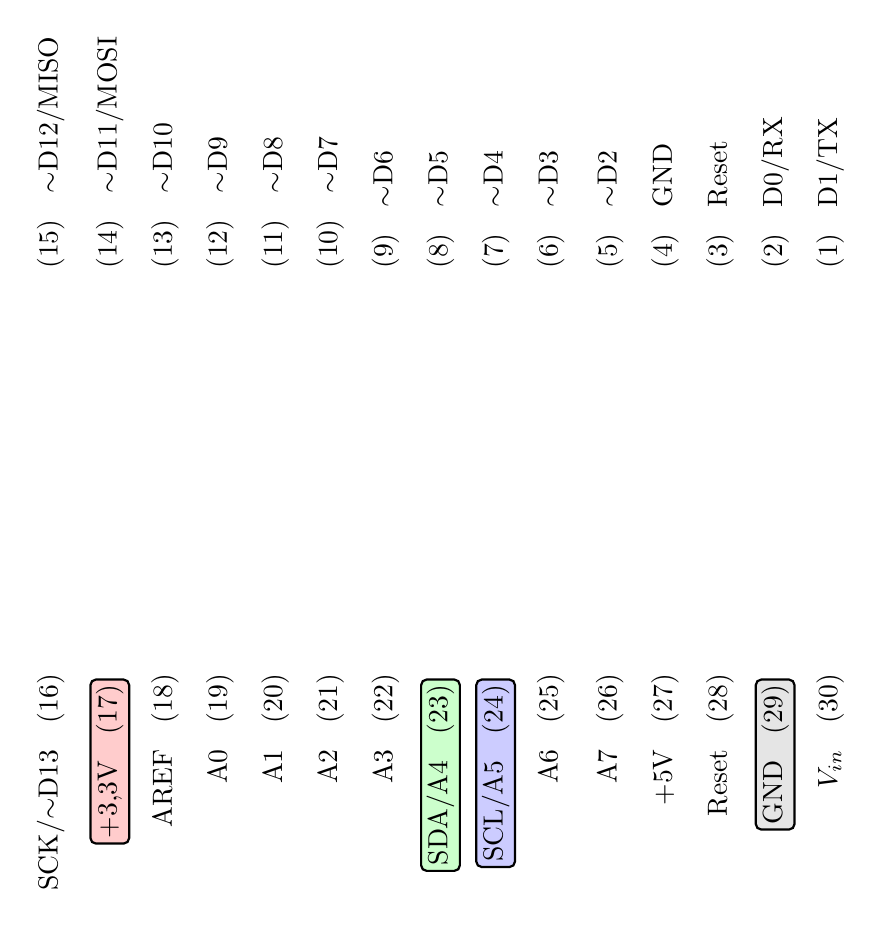
\begin{tikzpicture}
        
        \ArduinoNanoBLESenseLLite
        
        \node[rotate=90,right] (Pin1) at (11.2,4.9) {(1) \; D1/TX};
        \node[rotate=90,right] (Pin2) at (10.5,4.9) {(2) \; D0/RX};
        \node[rotate=90,right] (Pin3) at (9.8,4.9) {(3) \; Reset};
        \node[rotate=90,right] (Pin4) at (9.1,4.9) {(4) \; GND};
        \node[rotate=90,right] (Pin5) at (8.4,4.9) {(5) \; $\sim$D2};
        \node[rotate=90,right] (Pin6) at (7.65,4.9) {(6) \; $\sim$D3};
        \node[rotate=90,right] (Pin7) at (6.95,4.9) {(7) \; $\sim$D4};
        \node[rotate=90,right] (Pin8) at (6.25,4.9) {(8) \; $\sim$D5};
        \node[rotate=90,right] (Pin9) at (5.55,4.9) {(9) \; $\sim$D6};
        \node[rotate=90,right] (Pin10) at (4.85,4.9) {(10) \; $\sim$D7};
        \node[rotate=90,right] (Pin11) at (4.15,4.9) {(11) \; $\sim$D8};
        \node[rotate=90,right] (Pin12) at (3.45,4.9) {(12) \; $\sim$D9};
        \node[rotate=90,right] (Pin13) at (2.75,4.9) {(13) \; $\sim$D10};
        \node[rotate=90,right] (Pin14) at (2.05,4.9) {(14) \; $\sim$D11/MOSI};
        \node[rotate=90,right] (Pin15) at (1.3,4.9) {(15) \; $\sim$D12/MISO};
        
        
        \node[rotate=90,left] (Pin30) at (11.2,-0.0) { $V_{in}$ \; (30)};
        \node[rotate=90, left, fill=black!10, draw=black, thick, rounded corners=2pt, inner sep=2pt] (Pin1) at (10.5,-0.18) {GND \; (29)};
        \node[rotate=90,left] (Pin2) at (9.8,-0.0) {Reset \; (28)};
        \node[rotate=90,left] (Pin3) at (9.1,-0.0) {+5V \; (27)};
        \node[rotate=90,left] (Pin4) at (8.4,-0.0) {A7 \; (26)};
        \node[rotate=90,left] (Pin5) at (7.65,-0.0) {A6 \; (25)};
\node[rotate=90, left, fill=blue!20
, draw=black, thick, rounded corners=2pt, inner sep=2pt] (Pin6) at (6.95,-0.18) {SCL/A5 \; (24)};
\node[rotate=90, left, fill=green!20, draw=black, thick, rounded corners=2pt, inner sep=2pt] (Pin7) at (6.25,-0.18) {SDA/A4 \; (23)};
        \node[rotate=90,left] (Pin8) at (5.55,-0.0) {A3 \; (22)};
        \node[rotate=90,left] (Pin9) at (4.85,-0.0) {A2 \; (21)};
        \node[rotate=90,left] (Pin10) at (4.15,-0.0) {A1 \; (20)};
        \node[rotate=90,left] (Pin11) at (3.45,-0.0) {A0 \; (19)};
        \node[rotate=90,left] (Pin12) at (2.75,-0.0) {AREF \; (18)};
        \node[rotate=90, left, fill=red!20, draw=black, thick, rounded corners=2pt, inner sep=2pt] (Pin13) at (2.05,-0.18) {+3{,}3V \; (17)};
        \node[rotate=90,left] (Pin14) at (1.3,-0.0) {SCK/$\sim$D13 \; (16)};
        
    \end{tikzpicture}
    \caption{Verwendente Pins des Nano 33 BlE Sense Lite`s}
    \label{fig:Nano_Lite_Pinout}
\end{figure}

%\begin{figure}
%    \begin{center}
%        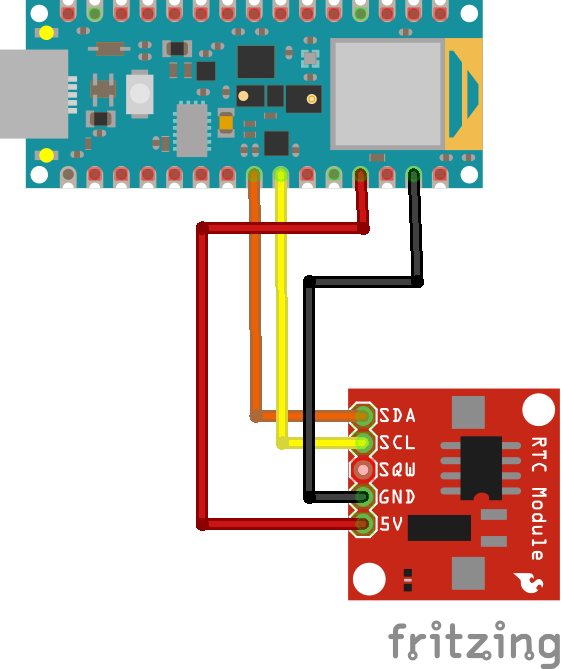
\includegraphics[width=8cm]{../../Images/RTC/Connecting.png}
%        \caption{Schaltplan Real Time Clock und Arduino Nano 33 BLE Sense Lite}
%        \label{fig:Schaltplan_RTC}
%    \end{center} 
%\end{figure}

%---------------------------------------------------------------------------------------------------------------------------%





%---------------------------------------------Bibliothek DS3231----------------------------------------------------------------------%




\section{Bibliothek \FILE{RTClib.h}}
\label{sec:bib_rtclib}

\subsection{Beschreibung der Bibliothek}

Für den Betrieb von Echtzeituhr-Modulen (\ac{rtc}) stehen verschiedene Arduino-Bibliotheken zur Verfügung. 
Eine weit verbreitete und aktiv gepflegte Bibliothek ist die \FILE{RTClib.h} von \PYTHON{Adafruit}, 
welche die Kommunikation mit Modulen, wie dem DS3231, über die I\textsuperscript{2}C-Schnittstelle ermöglicht \cite{Adafruit:2023}.

Die Bibliothek-\PYTHON{RTClib} unterstützt folgende RTC-Module:

\begin{itemize}
	\item DS3231
	\item DS1307
	\item PCF8523
\end{itemize}


\subsection{Installation}

Die Installation der Bibliothek erfolgt in der Arduino IDE-Umgebung, welche dafür zuerst einmal geöffnet werden muss. Ist dieser Schritt erfolgt, so kann die Bibliothek unter \menu{Sketch > Bibliothek einbinden > Bibliotheken verwalten} nach Abbildung \ref{fig:LibInstallation01} eingebunden werden.

\begin{figure}
	\begin{center}
		
\includegraphics[width=12cm]{RTC/LibExampleInstallation01.png}
		\caption{\FILE{RTClib.h} Installation Schritt 1}
		\label{fig:LibInstallation01}
	\end{center}
\end{figure}

Daraufhin öffnet sich die Bibliotheksverwaltung. 
In dieser muss, wie in Abbildung~\ref{fig:LibInstallation02} gezeigt, 
nach der Bibliothek-\PYTHON{RTClib} gesucht werden. 
Sobald die Bibliothek-\PYTHON{RTClib} des Herstellers \PYTHON{Adafruit} gefunden wurde, 
kann diese durch einen Mausklick auf \menu{Installieren} installiert werden. In dieser Darstellung (Abbildung~\ref{fig:LibInstallation02}) ist die zum Zeitpunkt der Installation aktuelle Version~2.1.4 der Bibliothek-\PYTHON{RTClib} gezeigt.

\begin{figure}
	\begin{center}
		
\includegraphics[width=12cm]{RTC/LibExampleInstallation02.png}
		\caption{\FILE{RTClib.h} Installation Schritt 2}
		\label{fig:LibInstallation02}
	\end{center}
\end{figure}

Falls die Bibliothek-\PYTHON{Adafruit BusIO}  noch nicht anderwertig installiert ist, 
erscheint ein Pop-up-Fenster, wie in Abbildung~\ref{fig:LibInstallation03} dargestellt. 
Die Bibliothek-\FILE{RTClib.h} ist von der Bibliothek-\PYTHON{Adafruit BusIO} abhängig, 
da sie deren grundlegende Kommunikationsfunktionen für die I\textsuperscript{2}C- und SPI-Kommunikation nutzt \cite{Adafruit:2023,Adafruit:2023b}. 
Um die Installation der Bibliothek-\FILE{RTClib.h} erfolgreich abzuschließen, 
muss daher auch die Bibliothek-\PYTHON{Adafruit BusIO} installiert werden. 
Im angezeigten Dialogfeld also auf \menu{Alle installieren} klicken.

\begin{figure}
	\begin{center}
		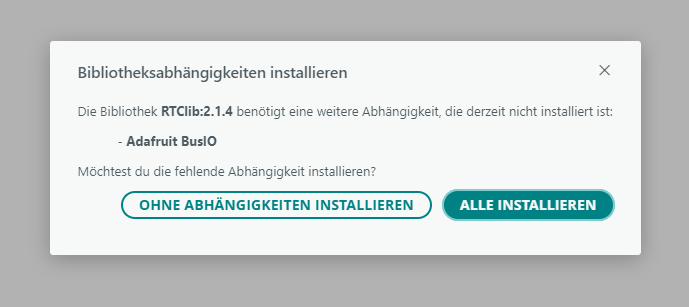
\includegraphics[width=12cm]{../../Images/RTC/LibInstallation03.png}
		\caption{\FILE{RTClib.h} Installation Schritt 3}
		\label{fig:LibInstallation03}
	\end{center}
\end{figure}

Danach erscheinen in der Ausgabe einige Meldungen \ref{fig:LibInstallation04} bezüglich des Downloads und der erfolgreichen Installation der Bibliotheken.

\begin{figure}
	\begin{center}
		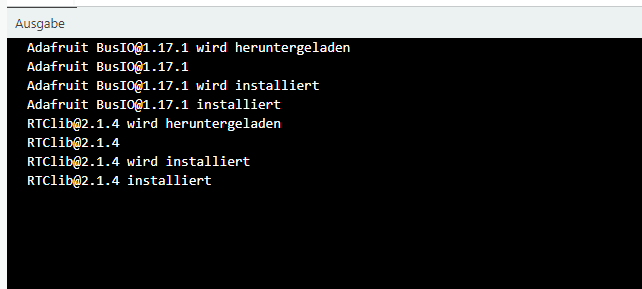
\includegraphics[width=12cm]{../../Images/RTC/LibInstallation04.png}
		\caption{\FILE{RTClib.h} Installation Schritt 4}
		\label{fig:LibInstallation04}
	\end{center}
\end{figure}

Nun können Beispielsketches der gewählten Bibliothek und dem gewählten Modul unter z.B. \menu{Datei > Beispiele > RTClib > ds3231} aufgerufen werden \ref{fig:LibExampleInstallation05}, welche die grundlegenden Funktionen dieser Bibliothek aufzeigt.

\begin{figure}
	\begin{center}
		
\includegraphics[width=12cm]{RTC/LibExampleInstallation05.png}
		\caption{\FILE{RTClib.h} Installation Schritt 5}
		\label{fig:LibExampleInstallation05}
	\end{center}
\end{figure}

\medskip

Zur Einbindung in einen Sketch müssen die folgenden Header-Dateien eingebunden werden:
\PYTHON{include <Wire.h>}  
\PYTHON{include "RTClib.h"}




Die Bibliothek-\FILE{Wire.h}  stellt die Funktionen für die I\textsuperscript{2}C-Kommunikation bereit, 
über die das RTC-Modul  mit dem Mikrocontroller kommuniziert \cite{ArduinoWire:2024}. 
Die darauf aufbauende Bibliothek-\FILE{RTClib.h} nutzt diese Kommunikationsschnittstelle, 
um den Zugriff auf Echtzeituhr-Module, wie dem DS3231, zu ermöglichen \cite{Adafruit:2023}.

Da die Bibliothek-\FILE{RTClib.h} intern auf die Funktionen der Bibliothek-\FILE{Wire.h} zugreift, 
ist die Einbindung beider Bibliotheken zwingend erforderlich.

\medskip

%-------------------------------------------------------Bib-Funktionen---------------------------------------------------------------------%

\newpage
\subsection{Funktionen}

Die Bibliothek-\FILE{RTClib.h} stellt mehrere Klassen zur Verfügung, über die Echtzeituhr-Module wie der DS3231 angesteuert werden können. 
Die Funktionen sind in drei Hauptklassen gegliedert: 
\PYTHON{RTC\_DS3231}, \PYTHON{DateTime} und \PYTHON{TimeSpan}. 
Die folgende Übersicht fasst die zentralen Funktionen zusammen.

% --- Tabelle 1: RTC_DS3231 ------------------------------------------------
\begin{table}[H]
	\centering
	\renewcommand{\arraystretch}{1.2}
	\caption{Funktionen der Klasse \PYTHON{RTC\_DS3231}~\cite{Adafruit:2023}}
	\label{tab:rtc_ds3231_functions}
	\begin{tabular}{|>{\centering\arraybackslash}p{4cm}|p{9cm}|}
		\hline
		\textbf{Funktion} & \textbf{Beschreibung} \\ \hline
		\PYTHON{begin()} & Initialisiert die Kommunikation mit dem RTC-Modul über die I\textsuperscript{2}C-Schnittstelle. \\ \hline
		\PYTHON{lostPower()} & Prüft, ob das RTC-Modul seit dem letzten Start einen Stromausfall hatte. \\ \hline
		\PYTHON{adjust(DateTime dt)} & Setzt das aktuelle Datum und die Uhrzeit des Moduls. \\ \hline
		\PYTHON{now()} & Gibt die aktuelle Zeit als \PYTHON{DateTime}-Objekt zurück. \\ \hline
		\PYTHON{getTemperature()} & Liefert die vom DS3231 intern gemessene Temperatur in Grad Celsius. \\ \hline
	\end{tabular}
\end{table}

\vspace{0.5cm}

% --- Tabelle 2: DateTime ------------------------------------------------
\begin{table}[H]
	\centering
	\renewcommand{\arraystretch}{1.2}
	\caption{Funktionen der Klasse \PYTHON{DateTime}~\cite{Adafruit:2023}}
	\label{tab:datetime_functions}
	\begin{tabular}{|>{\centering\arraybackslash}p{4cm}|p{9cm}|}
		\hline
		\textbf{Funktion} & \textbf{Beschreibung} \\ \hline
		\PYTHON{DateTime(year, month, day, hour, minute, second)} & Erstellt ein Zeitobjekt mit festen Datums- und Uhrzeitwerten. \\ \hline
		\PYTHON{year()}, \PYTHON{month()}, \PYTHON{day()} & Zugriff auf die einzelnen Datumswerte. \\ \hline
		\PYTHON{hour()}, \PYTHON{minute()}, \PYTHON{second()} & Zugriff auf die aktuelle Uhrzeit. \\ \hline
		\PYTHON{dayOfTheWeek()} & Gibt den Wochentag zurück (0 = Sonntag, 6 = Samstag). \\ \hline
		\PYTHON{unixtime()} & Wandelt das aktuelle Datum in einen Unix-Zeitstempel um (Sekunden seit dem 1.~Januar~1970). \\ \hline
	\end{tabular}
\end{table}

\vspace{0.5cm}

% --- Tabelle 3: TimeSpan ------------------------------------------------
\begin{table}[H]
	\centering
	\renewcommand{\arraystretch}{1.2}
	\caption{Funktionen der Klasse \PYTHON{TimeSpan}~\cite{Adafruit:2023}}
	\label{tab:timespan_functions}
	\begin{tabular}{|>{\centering\arraybackslash}p{4cm}|p{9cm}|}
		\hline
		\textbf{Funktion} & \textbf{Beschreibung} \\ \hline
		\PYTHON{TimeSpan(days, hours, minutes, seconds)} & Erstellt ein Zeitintervall, z.\,B. 3~Tage oder 5~Stunden. \\ \hline
		\PYTHON{total\_seconds()} & Gibt die Gesamtdauer des Zeitintervalls in Sekunden zurück. \\ \hline
		\PYTHON{DateTime + TimeSpan} & Berechnet einen zukünftigen Zeitpunkt basierend auf einem Zeitintervall. \\ \hline
		\PYTHON{DateTime - DateTime} & Ergibt den Zeitunterschied zweier Zeitpunkte als \PYTHON{TimeSpan}. \\ \hline
	\end{tabular}
\end{table}

\medskip
\noindent 

Diese Funktionen erlauben das Auslesen, Setzen und Berechnen von Zeitwerten sowie die Überwachung der Spannungsversorgung und der Temperatur des RTC-Moduls DS3231. 



%---------------------------------------------------------------------------------------------------------------------------%
%
%\subsection{Funktionen}
%
%Die \FILE{RTClib.h} bietet viele Funktionen, die in drei Klassen unterteilt werden können. Die erste Klasse ist dabei RTC-Chip-spezifisch, weshalb in dieser Auflistung der DS1307 verwendet wird.
%
%\begin{enumerate}
%    \item \PYTHON{RTC\_DS1307}: Verbindet sich mit einem DS1307 und bietet Methoden zur Steuerung
%    \begin{itemize}
%        \item \PYTHON{begin()} -- Initialisiert die RTC
%        \item \PYTHON{isrunning()} -- Prüft, ob die Uhr läuft
%        \item \PYTHON{adjust(DateTime dt)} -- Setzt die Uhrzeit
%        \item \PYTHON{now()} -- Gibt die aktuelle Zeit als DateTime zurück
%        \item \PYTHON{readSqwPinMode()} -- Liest die aktuelle Rechteckwellen-Einstellung
%        \item \PYTHON{writeSqwPinMode(mode)} -- setzt die Frequenz des SQW-Pins
%    \end{itemize}
%    \item \PYTHON{DateTime}: Kapselt ein Datum und eine Uhrzeit in einem Objekt und kann z.B. von \PYTHON{now()} zurückgegeben werden.
%    \begin{itemize}
%        \item Konstruktor: \PYTHON{DateTime(year, month, day, hour, minute, second)}
%        \item \PYTHON{year()}, \PYTHON{month()}, \PYTHON{day()} -- Zugriff auf das Datum
%        \item \PYTHON{hour()}, \PYTHON{minute()}, \PYTHON{second()} -- Zugriff auf die Uhrzeit
%        \item \PYTHON{dayOfTheWeek()} -- Wochentag (0 = Sonntag)
%        \item \PYTHON{unixtime()} -- Unix-Zeitstempel
%        \item \PYTHON{timestamp()} -- formatiertes Datum als String
%    \end{itemize}
%    \item \PYTHON{TimeSpan}: Dient zur Darstellung von Zeitintervallen (z.B. 3 Tage, 5 Stunden, etc.)
%    \begin{itemize}
%        \item Konstruktor: \PYTHON{TimeSpan(days, hours, minutes, seconds)}
%        \item \PYTHON{total\_seconds()} -- gibt die Gesamtdauer in Sekunden
%        \item \PYTHON{days()}, \PYTHON{hours()}, \PYTHON{minutes()}, \PYTHON{seconds()} -- Einzelwerte
%        \item Diese Daten können mit \PYTHON{DateTime} verrechnet werden:
%        \begin{itemize}
%            \item \PYTHON{DateTime} + \PYTHON{TimeSpan} \textrightarrow ~ zukünftiger Zeitpunkt
%            \item \PYTHON{DateTime} - \PYTHON{DateTime} \textrightarrow ~ ergibt \PYTHON{TimeSpan}
%        \end{itemize}
%    \end{itemize}
%\end{enumerate}

%---------------------------------------------------------------------------------------------------------------------------%



\section{Testen der Funktionen}
\label{sec:functiontest}

Um ein besseres Verständnis für die bereitgestellten Funktionen der Bibliothek-\FILE{RTClib.h} zu erhalten,
wurde ein einfacher Funktionstest erstellt. 
Dieser soll zeigen, wie grundlegende Befehle der Bibliothek in Kombination mit dem RTC-Modul DS3231 
verwendet werden können.

\subsubsection*{Beschreibung}

Ist das Modul korrekt über die I\textsuperscript{2}C-Schnittstelle mit dem Mikrocontroller verbunden 
und wird es erkannt, so liest der Mikrocontroller die aktuelle Uhrzeit und das Datum aus dem RTC-Modul aus.
Darüber hinaus wird die im DS3231 integrierte Temperaturmessung genutzt, 
um die aktuelle Temperatur des Moduls auszugeben.

Zusätzlich wird mit Hilfe der Klassen \PYTHON{DateTime} und \PYTHON{TimeSpan} 
der Bibliothek-\FILE{RTClib.h} die Anzahl der vergangenen Tage seit einem festgelegten Referenzdatum 
(21.~März~2021) berechnet.
Alle Ergebnisse werden im seriellen Monitor angezeigt und sind in Abbildung \ref{fig:functiontestoutcome} dargestellt: 
das aktuelle Datum, die Uhrzeit, die vergangene Zeitspanne in Tagen sowie die gemessene Temperatur werden ausgegeben.

Die Ausgabe erfolgt in einem festen Intervall von zehn Minuten, 
wodurch sich die Stabilität der Zeitmessung und die Temperaturwerte über längere Zeit beobachten lassen.

\begin{figure}
	\centering
	
\includegraphics[width=12cm]{RTC/DS3231FunctionTestOutcome}
	\caption{Ausgabe im Seriellen Monitor zum Funktionstest}\label{fig:functiontestoutcome}
\end{figure}

\medskip
\noindent

\subsubsection*{Code zum Testen der Funktionen}

Der in Listing~\ref{lst:RTC_Function_Test} dargestellte Sketch \FILE{functiontest.ino}
zeigt einen einfachen Funktionstest der zentralen Hauptfunktionen der Bibliothek-\FILE{RTClib.h}.


\begin{code}
	\ArduinoExternal{}{../../Code/Nano33BLESense/RTCDS3231/DS3231TestFunction/DS3231TestFunction.ino}
	\captionof{code}{Testen der \FILE{RTClib.h}-Funktionen} 
	\label{lst:RTC_Function_Test}
\end{code}





%Hierzu zählen das Auslesen der aktuellen Uhrzeit und des Datums, 
%die Berechnung der vergangenen Tage seit einem festgelegten Referenzdatum 
%sowie die Messung der im Modul integrierten Temperatur.



%\section{Testen der Funktionen}
%
%Um eine bessere Vorstellung von den aufgelisteten Funktionen der \FILE{RTClib.h}-Bibliothek zu erhalten wird im folgenden ein Code beschrieben, welcher diese testen soll.
%
%\subsection{Beschreibung}
%
%Ist das Modul korrekt angeschlossen und vom Mikrocontroller erkannt worden, so wird zuerst die aktuelle Systemzeit aus dem RTC-Modul ausgelesen und in verschiedenen Formaten dargestellt: Als strukturierte Einzelwerte (Jahr, Monat, Tag, Stunde, Minute, Sekunde), als formatierter Zeitstempel-String, sowie als Unix-Zeitwert (Sekunden seit dem 1. Januar 1970).
%\\
%Zur Demonstration zeitlicher Operationen wird zudem mithilfe der \PYTHON{TimeSpan}-Klasse ein zukünftiger Zeitpunkt berechnet, indem der aktuellen Uhrzeit eine definierte Zeitspanne von drei Tagen und zwei Stunden addiert wird.
%
%\subsection{Code zum Testen der Funktionen}
%
%Der Code \ref{lst:RTC_Function_Test} zeigt das entsprechende Programm zum Testen einiger Funktionen.
%
%{
%    \captionof{code}{Testen der \FILE{RTClib.h}-Funktionen} \label{lst:RTC_Function_Test}
%    \ArduinoExternal{}{../../Code/Arduino/RTC/DS3231TestFunction/DS3231TestFunction.ino}
%}
%
%%\begin{code}
%%	\ArduinoExternal{}{../../Code/Arduino/RTC/rtc_function_test/rtc_function_test.ino}
%%	\label{Code:RTC_Function_Test}
%%	\caption{Testen der \FILE{RTClib.h}-Funktionen}
%%\end{code}

%---------------------------------------------------------------------------------------------------------------------------%

\medskip
\noindent

\newpage


\section{Einfacher Code}
\label{sec:rtc_simple}

Über die Bibliothek-\FILE{RTClib.h} kann die Ausgabe des Zeitstempels in unterschiedlichen Formaten erfolgen. 
Um eine einheitliche und systemübergreifende Darstellung zu gewährleisten, 
wird im Folgenden ein standardisiertes Format gewählt und durch den einfachen Code ausgegeben. 
Der Zeitstempel folgt dem international genormten ISO~8601-Format \cite{ISO8601:2019} 
und besteht aus dem vollständigen Datum sowie der Uhrzeit in Stunden, Minuten und Sekunden. 
Durch die Ausgabe der Meldung, dass das Modul initialisiert wurde, 
wird gleichzeitig bestätigt, dass das RTC-Modul DS3231 erfolgreich über die I\textsuperscript{2}C-Schnittstelle 
mit dem Mikrocontroller Nano~33~BLE~Sense~Lite kommuniziert und der Datenaustausch ordnungsgemäß funktioniert. 

Ein einheitlicher Zeitstempel ist besonders wichtig, um die Konsistenz bei der Weiterverarbeitung 
von Zeitinformationen in anderen Modulen sicherzustellen. 
Der einfache Code ist modular aufgebaut und besteht aus einer \FILE{RTC\_Module.h}-, 
einer \FILE{RTC\_Module.cpp}- sowie der Hauptdatei \FILE{functiontest.ino}. 
Die Erzeugung des Zeitstempels erfolgt innerhalb der Funktion \PYTHON{rtc\_getTimestamp()}, 
während die Ausgabe im seriellen Monitor über die Funktion \PYTHON{rtc\_sendMessage()} realisiert wird. 
In späteren Erweiterungen kann diese Funktion angepasst werden, 
um die Ausgabe zusätzlich in eine CSV-Datei zu schreiben. 

 
Die Ausgabe des Zeitstempels im seriellen Monitor ist in Abbildung~\ref{fig:simplecode_output} dargestellt.

\medskip
\noindent

 \begin{figure}
	\centering
	
\includegraphics[width=0.8\linewidth]{RTC/SimpleCodeDS3231Outcome.png}
	\caption{Einfacher Code: Zeitstempel-Ausgabe im Seriellen Monitor}
	\label{fig:simplecode_output}
\end{figure}

\newpage

Das Listing~\ref{lst:simplecodeds3231} zeigt den einfachen Anwendungscode zur Ausgabe 
eines standardisierten Zeitstempels über das RTC-Modul DS3231.


\begin{code}
	\caption{Zeitstempel}
	\label{lst:simplecodeds3231}
	\ArduinoExternal{
	}{../../Code/Nano33BLESense/RTCDS3231/SimpleCodeDS3231/SimpleCodeDS3231.ino}
\end{code}

\Mynote{Hier fragen wegen Klassen und Objekten... Variante 2 existiert auch aber welche möchten Sie haben?}





%---------------------------------------------------------------------------------------------------------------------------%


\newpage

\section{Einfache Anwendung }
\label{sec:rtc_application}

In der folgenden Anwendung wird die Funktionsweise des RTC-Moduls~DS3231 im Zusammenhang 
mit der integrierten Backup-Batterie untersucht. 
Das Modul soll auch bei einem Stromausfall die gespeicherte Zeitinformation beibehalten. 
Über die Bibliothek-\FILE{RTClib.h} werden die benötigten Funktionen bereitgestellt, 
um den Zustand des RTC-Moduls und die aktuelle Uhrzeit auszulesen. 
Die Anwendung ist modular aufgebaut und in drei Dateien unterteilt: 
\FILE{SampleDS3231.ino}, \FILE{RTC\_LostPower.cpp} und \FILE{RTC\_LostPower.h}.

\subsubsection*{\FILE{SampleDS3231.ino}}

Die Datei \FILE{SampleDS3231.ino} enthält das Hauptprogramm zur Steuerung des RTC-Modul DS3231. 
Nach dem Start des Mikrocontrollers wird das RTC-Modul mit der Funktion \PYTHON{rtc\_init()} gestartet. 
Dabei prüft das Programm, ob das Modul angeschlossen ist und ob ein Stromausfall erkannt wurde. 
Wenn ein Energieverlust festgestellt wird, erscheint im seriellen Monitor die Meldung 
\enquote{RTC lost power -> manual time adjustment required}.

In diesem Fall muss die aktuelle Uhrzeit in der Datei \FILE{RTC\_LostPower.cpp} 
einmalig mit dem Befehl:
\begin{center}
	\PYTHON{rtc.adjust(DateTime(YYYY, MM, DD, hh, mm, ss));}
\end{center}
manuell eingetragen werden. 
Nach dem Hochladen des Programms kann diese Zeile wieder auskommentiert werden. 
Solange die Backup-Batterie funktioniert, behält das RTC-Modul danach ihre Zeit. 
Wenn kein Energieverlust erkannt wird, zeigt das Programm die Meldung 
\enquote{RTC running normally.~Time preserved}.

Im weiteren Verlauf gibt das Programm mit der Funktion \PYTHON{rtc\_sendMessage()} 
regelmäßig den aktuellen Zeitstempel (vgl. Abbildung \ref{fig:sampleds3231_output}) aus. 
So kann überprüft werden, ob die RTC korrekt arbeitet und die Zeit fortlaufend aktualisiert wird.

\subsubsection*{\FILE{RTC\_LostPower.cpp}}
Die Datei \FILE{RTC\_LostPower.cpp} enthält die Funktionen zur Umsetzung der Echtzeituhr. 
Mit \PYTHON{rtc.begin()} wird die Kommunikation mit dem DS3231-Modul über den I\textsuperscript{2}C-Bus hergestellt.
Danach prüft \PYTHON{rtc.lostPower()}, ob die Uhr ihre Stromversorgung verloren hat. 
Je nach Ergebnis zeigt das Programm eine passende Meldung im seriellen Monitor an: 
\enquote{RTC lost power~$\rightarrow$~manual time adjustment required} 
oder 
\enquote{RTC running normally.~Time preserved}.

Wenn die Uhrzeit neu eingestellt werden muss, kann dies in dieser Datei 
mit dem Befehl \PYTHON{rtc.adjust()} gemacht werden. 
Die Funktion \PYTHON{rtc\_getTimestamp()} liest die aktuelle Zeit aus 
und gibt sie als String, also als Zeichenkette, im ISO~8601-Format zurück \cite{ISO8601:2019} . 
Ein Beispiel für die Ausgabe ist:

\begin{center}
	\enquote{2025-11-03T16:45:25}.
\end{center}

\subsubsection*{\FILE{RTC\_LostPower.h}} 

In der Headerdatei \FILE{RTC\_LostPower.h} sind die Funktionen definiert. 
\PYTHON{rtc\_init()} dient zur Initialisierung des Moduls, 
\PYTHON{rtc\_getTimestamp()} erzeugt den formatierten Zeitstempel 
und \PYTHON{rtc\_sendMessage()} gibt den Zeitstempel über den seriellen Monitor aus. 
Die Funktionen sind modular aufgebaut und können unverändert in andere Anwendungen übernommen werden. 

Das Listing~\ref{lst:simpleapplicationds3231} zeigt den vollständigen Programmcode der einfachen Anwendung. 
Die resultierende Ausgabe im seriellen Monitor ist in Abbildung~\ref{fig:sampleds3231_output} dargestellt.

\begin{code}
	\captionof{code}{Einfache Anwendung zur Erkennung eines Energieverlustes der RTC} 
	\label{lst:simpleapplicationds3231}
	\ArduinoExternal{}{../../Code/Nano33BLESense/RTCDS3231/SampleDS3231/SampleDS3231.ino}
\end{code}


\begin{code}
	\captionof{code}{Einfache Anwendung:\FILE{RTC\_LostPower.h}}
	\label{lst:LostPower.h}
	\ArduinoExternal{}{../../Code/Nano33BLESense/RTCDS3231/SampleDS3231/RTC\_LostPower.h}
\end{code}


\begin{code}
	\captionof{code}{Einfache Anwendung: \FILE{RTC\_LostPower.cpp} }
	\label{lst:LostPower.cpp}
	\ArduinoExternal{}{../../Code/Nano33BLESense/RTCDS3231/SampleDS3231/RTC\_LostPower.cpp}
\end{code} 

 \begin{center}
	
\includegraphics[width=0.8\linewidth]{RTC/SampleDS3231Outcome.png}
	\captionof{figure}{Einfache Anwendung: Zeitstempel-Ausgabe im Seriellen Monitor}
	\label{fig:sampleds3231_output}
\end{center}


%Der vorliegende Code \ref{lst:Simple_Application_RTC} zeigt ein einfaches Anwendungsbeispiel einer RTC. Ziel ist es, analoge Pulswerte von einem angeschlossenen Sensor einzulesen, mit einem aktuellen Zeitstempel zu versehen und die daraus resultierenden Datensätze auf einer SD-Karte abzuspeichern.
%\\
%Im \PYTHON{setup()}-Teil werden zunächst die RTC und das SD-Karten-Modul initialisiert. Die eigentliche Anwendung erfolgt im \PYTHON{loop()}. In regelmäßigen Abständen von einer Sekunde wird der aktuelle Analogwert des Pulssignals eingelesen und gemeinsam mit dem aktuellen Zeitstempel zu einem String zusammengeführt. Dieser besteht aus einem ISO-zeitformatierten Wert (YYYY-MM-DDTHH:MM:SS) und dem Messwert, getrennt durch ein Semikolon. Die Ausgabe erfolgt im Nachhinein über den seriellen Monitor und als Eintrag in einer Textdatei auf der SD-Karte.
%\\
%Dabei sind Zeitformatierung und Dateioperationen jeweils in eigene Funktionen gefasst, sodass es einfacher fällt das Modul zu erweitern.

%\clearpage

